\section{Modelo de C�mera}
As c�meras s�o modeladas como c�meras de pequenos orif�cios como mostrada na
imagem~\ref{fig:camera01}.Esse modelo define a proje��o b�sica

 This model defines
the basic projective imaging geometry with which the object landmarks are mapped onto
the 2D image plane. This model is a simplification of the optics of a real camera and
is used often in computer graphics and computer vision to describe the formation of
images in a camera. There are different ways of setting up the coordinate systems;
we use a right-handed coordinate system, where the center of projection is at the origin
and the image plane is at a distance f (focal length) away from it. ref[3]





\begin{figure}[h!]
\centering
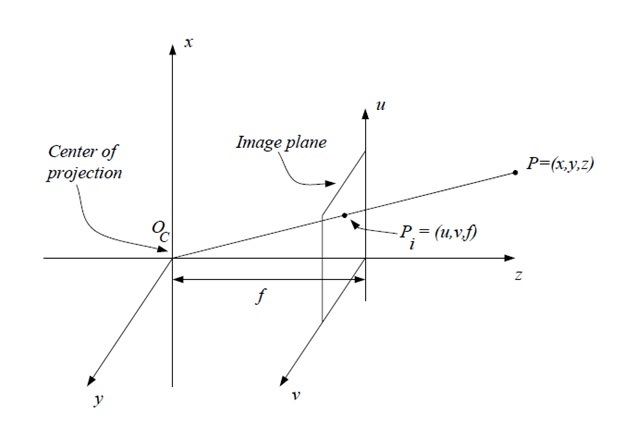
\includegraphics[scale=0.8]{images/camera01}
\caption{Camera no espa�o vetorial.}
\label{fig:camera01}
\end{figure}

\subsection{Calibra��o da C�mera}

Visto que as c�meras atuais adicionam distor��es, se faz necess�rio normalizar as
 imagens antes de utiliz�-las para que os pontos de refer�ncia n�o distor�am tanto na imagem como um todo,
  podendo sofrer efeitos de distor��o nas bordas por exemplo.
Considerando um modelo matem�tico que corrija as distor��es radiais e tangenciais. 
Para corrigir o fator radial, consideramos a seguinte transformada
\begin{figure}[h!]
\centering
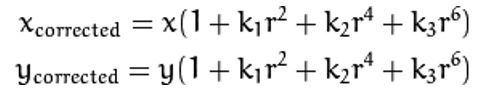
\includegraphics[scale=0.8]{images/camera_eq01}
\caption{Transforma��o de coordenadas}
\label{fig:camera_eq01}
\end{figure}


Em que (x,y) s�o a posi��o do ponto na imagem distorcida,
k1,k2 e k3 s�o constantes a serem descobertas pelo m�todo de calibra��o
r
Para corrigir a distor��o tangencial because image taking lense is not aligned perfectly parallel to the imaging plane.
 So some areas in image may look nearer than expected. It is solved as below:
 
 \begin{figure}[h!]
\centering
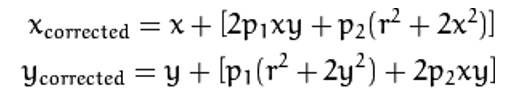
\includegraphics[scale=0.8]{images/camera_eq02}
\caption{Transforma��o de coordenadas quanto � distor��o radial}
\label{fig:camera_eq02}
\end{figure}

Para corrigirmos os dois efeitos e obtermos uma imagem calibrada temos que
resolver a matrix da imagem~\ref{fig:camera_eq03}

 
 \begin{figure}[h!]
\centering
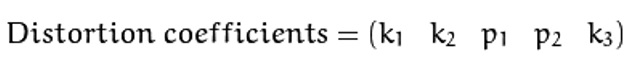
\includegraphics[scale=0.8]{images/camera_eq03}
\caption{Matriz de distor��es}
\label{fig:camera_eq03}
\end{figure}


